
\documentclass{article}

\usepackage{graphviz}
\usepackage{url}
\usepackage{hyperref}
\usepackage{fullpage}
\usepackage{parskip}
\usepackage{fancyvrb}
\usepackage{amsmath}
\usepackage[section]{placeins}
\usepackage{tikz-timing}

\usepackage{listings}
\lstset{numbers=left,
		basicstyle=\footnotesize,
		captionpos=b,
		xleftmargin=0.3in}

\usepackage[backend=biber,autocite=footnote,
	            bibstyle=authortitle,citestyle=verbose-inote]{biblatex}
\addbibresource{refs.bib}
\setlength\bibitemsep{1em}

\usepackage[xindy,toc,nonumberlist]{glossaries}
\makeglossaries
\renewcommand*{\glspostdescription}{}

\providecommand{\e}[1]{\ensuremath{\times 10^{#1}}}

\VerbatimFootnotes

\raggedright

\begin{document}

\nocite{github_jmahler_sprinklerpi}

% {{{ glossary entries

\newglossaryentry{SPI}
{
	name={SPI},
	description={Serial peripheral interface}.
}

\newglossaryentry{MOSI}
{
	name={MOSI},
	description={(SPI) master out slave in}.
}

\newglossaryentry{MISO}
{
	name={MOSI},
	description={(SPI) master in slave out}.
}

\newglossaryentry{GPIO}
{
	name={GPIO},
	description={General purpose input/output}.
}

\newglossaryentry{FIFO}
{
	name={FIFO},
	description={First in first out}.
}

% }}}

% {{{ title page
\vspace*{1.0in}

\centerline{\LARGE \textbf{SprinklerPI}}
\vspace{0.3in}
\centerline{\LARGE Product Design}

\vfill

\begin{center}
\begin{tabular}{c}
Jeremiah Mahler \\
EECE 490B, CSU Chico \\
May 6, 2014
\end{tabular}
\end{center}

\vspace{2in}

\thispagestyle{empty}

\pagebreak
% }}}

\nocite{rasberrypi}
\thispagestyle{empty}
\tableofcontents

% {{{ Architectural Design
\clearpage
\section{Architectural Design}

SprinklerPI is a web based sprinkler control system.
At the highest level it provides a web interface
which allows watering schedules to be created and modified.
To serve this web interface requires a web server.
In this case a web server running on Linux is used.

Each control/driver module can drive eight sprinkler valves.
And they accepts commands sent over SPI.
They can also be daisy chained together to drive more valves.
Since the RasberryPI can communicate over SPI it also
acts as the master of the SPI bus and sends these commands.

Between the web server and the SPI device both queuing and scheduling
must be performed.
A web server is not suited for these tasks because it is request driven.
To bridge this gap a set of daemons are provided.
Each one handles a specific tasks such as scheduling or queuing.

The communication channel between the web server and the daemons is the
file system.
A specific set of files at specific locations stores the entire state
of the system.
And these files are all in human readable format so they
can be accessed using standard command line tools.

And to power all of these devices requires a power supply capable
of providing both 24 volts AC and 3.3 volts DC.

Figure \ref{fig:spioview} shows an overview of the system.

\begin{figure}[h!]
\begin{center}
\includegraphics[scale=0.40]{dia/sprinklerpi_overview}
\end{center}
\caption{Overview of main components inside the SprinklerPI system.}
\label{fig:spioview}
\end{figure}

\pagebreak
When this system is installed on a private network or behind a firewall
it cannot be accessed from the Internet.  With the addition of a
client/server water daemon, that acts as a proxy, this system can still be
used as shown in Figure \ref{fig:spioviewnet}.

\begin{figure}[h!]
\begin{center}
\includegraphics[scale=0.40]{dia/sprinklerpi_overview-net}
\end{center}
\caption{SprinklerPI system configured for access behind a firewall.}
\label{fig:spioviewnet}
\end{figure}

% }}}

% {{{ Hardware Design
\clearpage
\section{Hardware Design}
\label{sec:hardware}

There are three main hardware components in this system:
the power supply, the Linux computer, and the control/driver.
Figure \ref{fig:hwoview} gives an overview of the hardware in the system.

\begin{figure}[h!]
\begin{center}
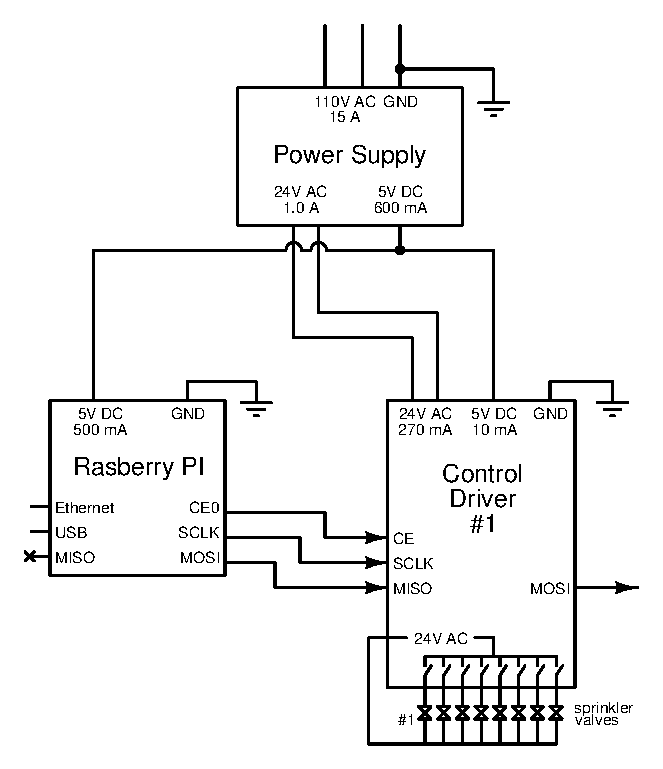
\includegraphics[scale=0.9]{xcircuit/hardware_overview}
\end{center}
\caption{Overview of hardware in system.
Only one control/driver is shown, 
additional control/drivers can be added up to a maximum of three.}
\label{fig:hwoview}
\end{figure}

The power supply takes 24 volts AC and outputs 3.3 volts DC
and 24 volts AC..
The 3.3 volts DC is used by the digital logic and the Linux computer.
The 24 volts AC is used to driver the sprinkler valves.
The power supply also includes an in line fuse to limit the current in
the AC circuit.

The Linux computer is a RasberryPI model B.
It communicates over Ethernet or using a wireless adapter.
And it communicates to the control/driver modules using SPI.

The control/driver accepts commands over SPI to turn on a particular valve.
It then switches the 24 volts AC supply using a triac to turn on a valve.
The control/driver can also be daisy chained to expand it up to a maximum
of three control/drivers.

\pagebreak

% {{{ State Flow Diagrams
\subsection{State Flow Diagrams}

The control/driver goes through two states as shown
in Figure \ref{fig:hwoview}.
When it is not receiving a command it is in the drive state.
In this state it is decoder is enabled and it is either driving
a valve or all valves are off.
In the receive command state the output decoder is disabled to
prevent incorrect intermediate states during transfer.
When it is disabled it will retain its previous value.
When the reception of a command over SPI is complete, the decoder
is re-enabled.

\begin{figure}[h!]
\centering
\includegraphics[scale=0.40]{dia/hardware_state}
\caption{State diagram of control/driver.}\label{fig:hwstate}
\end{figure}

% }}}

% {{{ Schematics
\clearpage
\FloatBarrier
\subsection{Schematics}

% {{{ Control
\FloatBarrier
\subsubsection{Control}
\label{sec:control}

The control part of the control/driver module interprets the commands
received over SPI which determines which valve will be driven or whether
they will be all off.
The driver will be discussed in more detail in Section \ref{sec:driver}.

Typical sprinkler systems can drive valves in groups of eight where only
one valve can be on at a
time\footnote{If multiple circuits were active this could lower the
water pressure resulting in inconsistent watering amounts.}.
This control module achieves this constraint in hardware by using a
decoder chip which only allows one output to be on at a time.

SPI is used to communicate between the Linux computer and the control
module.
Each module uses a 4-bit shift register but a minimum of 8-bits must
be sent per message from the Linux computer.
Additionally, when control/driver modules are daisy chained, more than
8-bits must be sent.

Figure \ref{fig:spi} shows the message format that is used.
Notice that there is a dedicated enable bit and it is active low.
Only 4-bits are used to address the valve.

{
\renewcommand*\arraystretch{1.5}
\begin{figure}[hbp]

\centering

\begin{tabular}{l r l r l r }
7 & 4 & 3 & 1 & \multicolumn{2}{c}{0} \\
\hline
\multicolumn{2}{|c|}{\hspace*{6mm} unused \hspace*{6mm}} &
\multicolumn{2}{|c|}{\hspace*{4mm} valve (group \#1) \hspace*{4mm}} &
\multicolumn{2}{|c|}{\hspace*{1mm} en\_n \hspace*{1mm}} \\
\hline
\end{tabular} \\
(a)

\begin{tabular}{l r l r l r l r }
7 & 5 & \multicolumn{2}{c}{4} & 3 & 1 & \multicolumn{2}{c}{0} \\
\hline
%\multicolumn{2}{|c|}{\hspace*{6mm} unused \hspace*{6mm}} &
\multicolumn{2}{|c|}{\hspace*{4mm} valve (group \#2) \hspace*{4mm}} &
\multicolumn{2}{|c|}{\hspace*{1mm} en\_n \hspace*{1mm}} &
\multicolumn{2}{|c|}{\hspace*{4mm} valve (group \#1) \hspace*{4mm}} &
\multicolumn{2}{|c|}{\hspace*{1mm} en\_n \hspace*{1mm}} \\
\hline
\end{tabular} \\
(b)

\caption{SPI message format for one group (a) and two groups (b).
Each group represents eight valves so (b) would support 16 valves.}
\label{fig:spi}
\end{figure}
}

Interpreting the message received is performed using a shift register
and decoder as shown in Figure \ref{fig:control}.
An output high of the decoder will turn on a valve.
Notice that the enable bit in the message will be output on \verb+OA+
which will enable the decoder chip.

\begin{figure}[hbp]
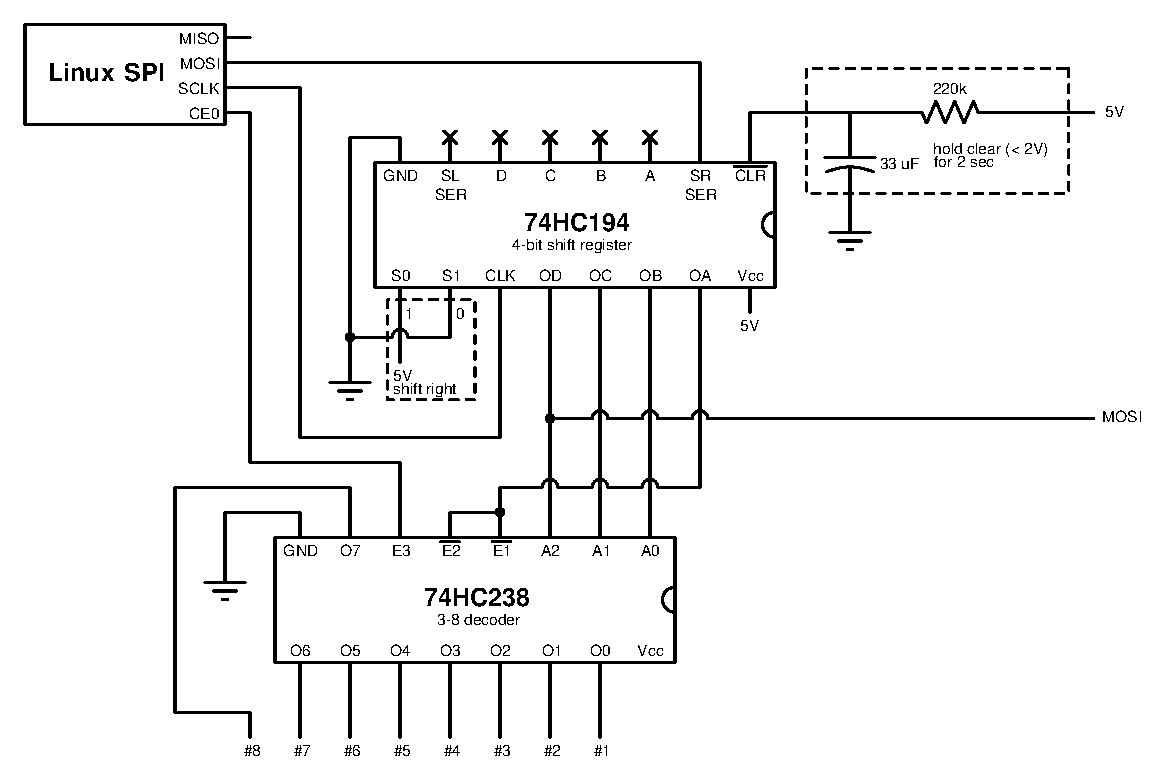
\includegraphics[scale=0.85]{xcircuit/control}
\caption{Sprinkler valve control logic.
Sprinkler valve number is input using SPI from the Linux computer in
to the shift register.
A 4-bit number is output from the shift register and sent to the
decoder which will turn on a valve or turn them all off.
All outputs are disabled when OA is clear.}\label{fig:control}
\end{figure}

% }}}

% {{{ Expansion
\clearpage
\subsubsection{Expansion}
\label{sec:expansion}

Each control/driver module accepts a command over SPI.
And depending on the message it receives it will turn one of the
eight valves on or turn them all off.
Up to three of these modules can be daisy chained together
to expand the system to a maximum of 24 valves.
This configuration is shown in Figure \ref{fig:expansion_spi}.

\begin{figure}[hbp]
\centering
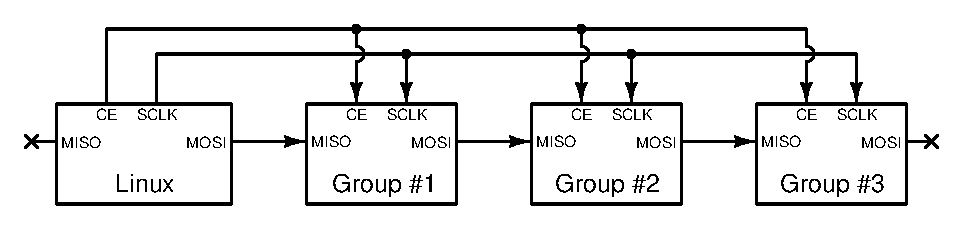
\includegraphics[angle=0,scale=0.80]{xcircuit/expansion_spi}
\caption{Daisy chain SPI configuration for multiple control groups.
}\label{fig:expansion_spi}
\end{figure}

The expansion of the current design is limited by the power supply.
It can only supply enough current to support three control/driver modules
and one Linux computer.
Figure \ref{fig:expansion_current} gives an overview.

\begin{figure}[hbp]
\centering
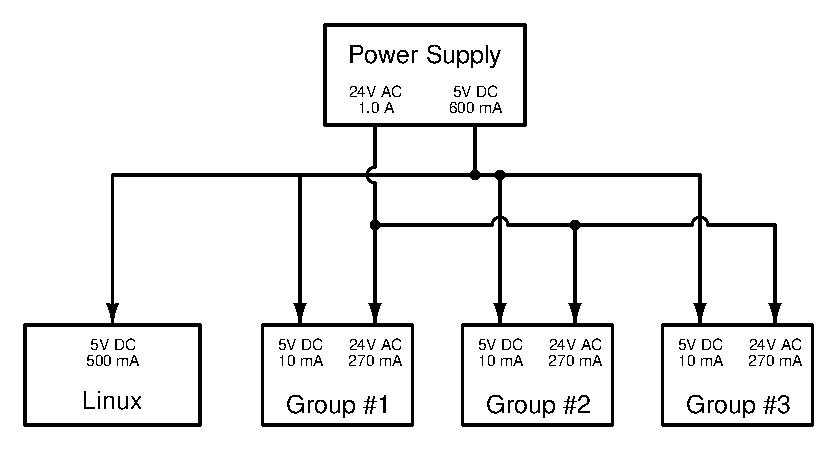
\includegraphics[angle=0,scale=0.80]{xcircuit/expansion_current}
\caption{With a power supply capable of 1 amp at 24 volts AC and
600 mA at 3.3 volts DC a maximum of three control groups and one
Linux computer can be driven.}\label{fig:expansion_current}
\end{figure}

% }}}

\pagebreak

% {{{ Driver
\FloatBarrier
\subsubsection{Driver}
\label{sec:driver}

The control part of the control/driver module (Section \ref{sec:control})
determines which valve will be driven.  But it cannot drive the valves
directly as they require 24 volts AC and the control circuit outputs
3.3 volts DC.
The purpose of the driver part of the control/driver module is to convert
these digital signal and drive the valves.
The driver circuitry is shown in Figure \ref{fig:driver}.

\begin{figure}[hbp]
\centering
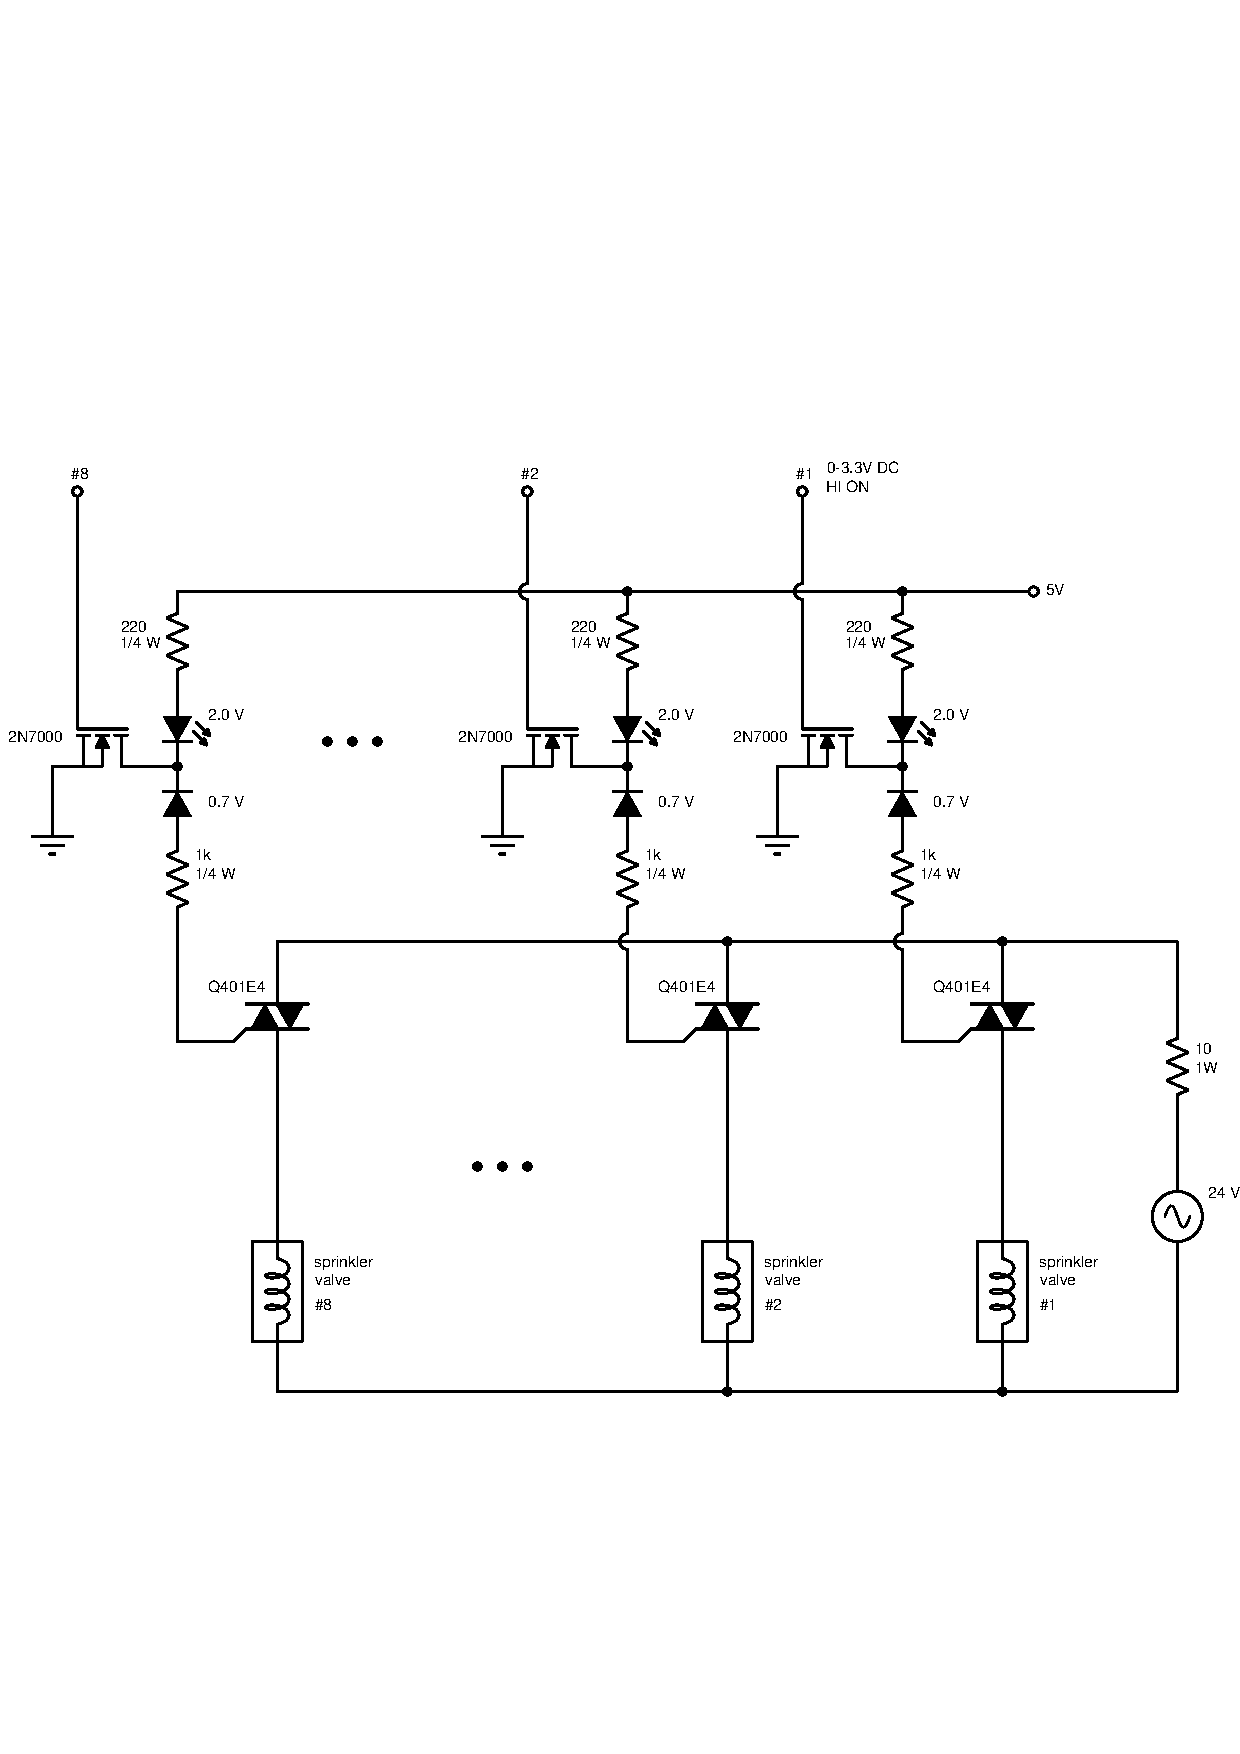
\includegraphics[scale=0.7]{xcircuit/driver_mult}
\caption{Sprinkler valve driver circuits.
Not all branches are shown since they are identical.
LEDs are used to indicate when the valve is on/off.
It is assumed that only one valve will be on at a time.}\label{fig:driver}
\end{figure}

To turn the sprinkler valves on requires 24 volts AC at approximately 270 mA.
Each sprinkler valve has a resistance of approximately 80 $\Omega$.
A 10 $\Omega$ resistor was added to limit the current to 270 mA.
A resistor with a 1 watt rating provides over a 10\% operating margin.

\begin{align*}
	P &= I^2 R \\
	  &= (270\e{-3})^2 \cdot 10 \\
	  &= 0.729 \quad \text{[W]}
\end{align*}

The control signal to the triac (Q401E4) is very sensitive.
The tiniest of currents in either direction will turn it on.
A diode is used to restrict the current to one direction and ensure
that the triac will switch off.
The FET (2N7000) drives the triac as well as the LED indicator.
It also serves to limit the gate current required from the control module.
The required gate current is less than 0.5 mA which is well within
the limits of CMOS logic used by the control module (Section \ref{sec:control}).

% }}}

% {{{ Power Supply
\subsubsection{Power Supply}
\label{sec:power}

The power supply must provide two different voltages: 24 volts AC and
3.3 volts DC.
The sprinkler valves require 24 volts AC at 270 mA.
The Linux computer and other digital logic require 3.3 volts DC with a
maximum draw of 600 mA
\footnote{The current draw of the RasberryPI was determined
experimentally to be approximately 500 mA.}.
These voltages must be created from a 24 volt AC input.
The 24 volts AC is converted from 110 volts AC using a transformer.
Plug mounted 110 to 24 volts AC transformers are commonly available
as most sprinkler controllers use these.

A switching voltage regulator, the MC34063A, was chosen for
the 3.3 volt supply.
It has a greater efficiency than a linear regulator such as
the LM7805.

The circuit which achieves all of these design requirements is
shown in Figure \ref{fig:power}.

\begin{figure}[hbp]
\centering
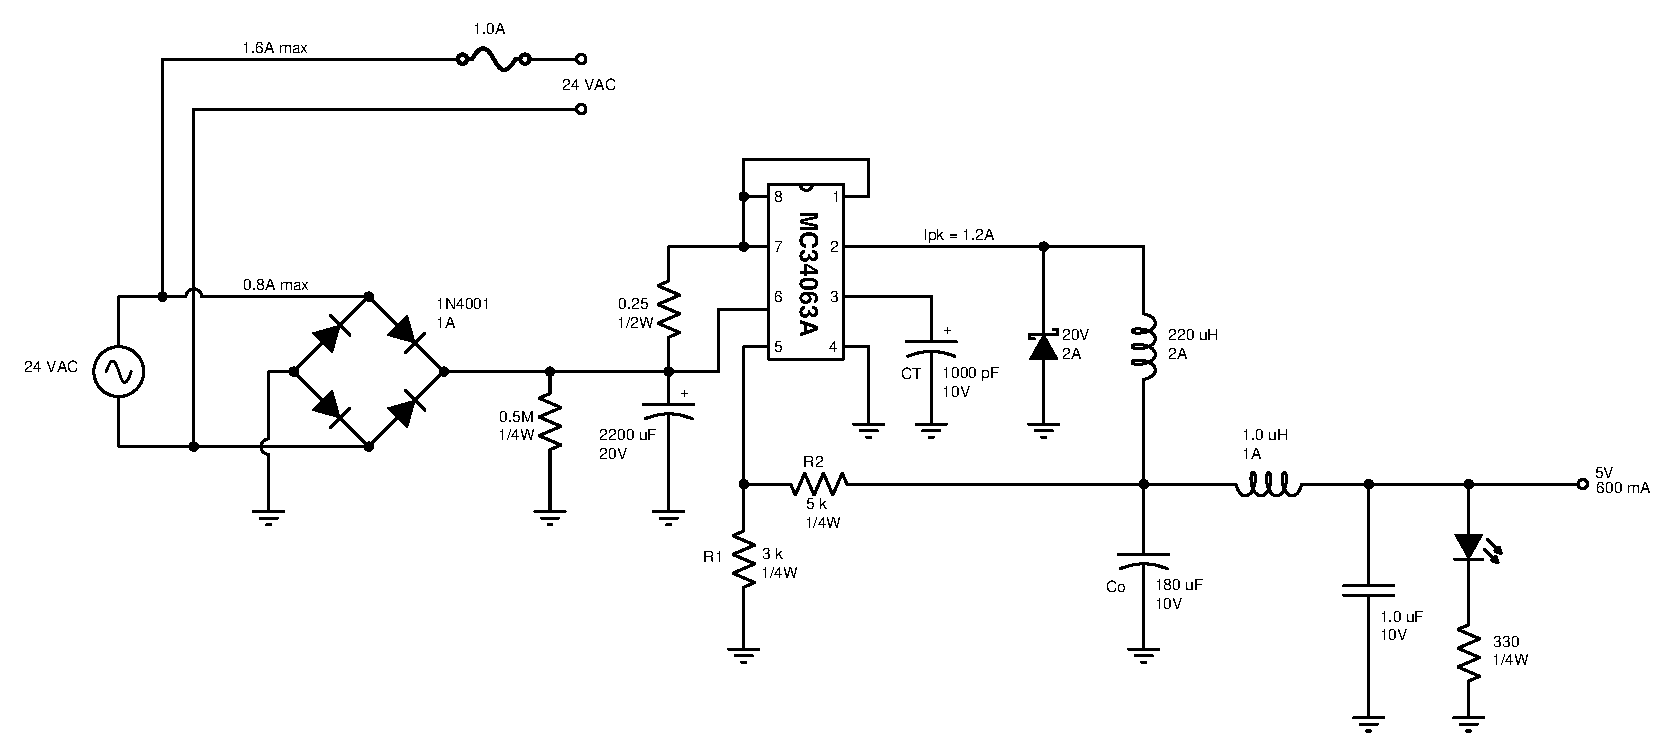
\includegraphics[angle=90,scale=0.70]{xcircuit/power_supply}
\caption{Power supply circuit. A 24 volt AC and 3.3 volt DC output are
provided.  The 3.3 volt DC is provided by the MC340363A switching
regulator.}\label{fig:power}
\end{figure}

% }}}

% }}}

% {{{ Timing Diagrams
\FloatBarrier
\subsection{Timing Diagrams}

Figure \ref{fig:timing} is a diagram of a message being sent
using SPI from the Linux computer to the control module.
Refer to Section \ref{sec:control} for a description of
the meaning of these messages.

\begin{figure}[h!]
\begin{center}
\begin{tikztimingtable}
	[xscale=2.0, yscale=2.0]
	CE	 & {1H} 1{C} {12L} 1{C} {1H} \\
	SCLK & {1H} 14{C} {1H} \\
	MOSI & 10L 1{C} 1{H} 1{C} 3L \\
	MISO & 16L \\
\end{tikztimingtable}
\end{center}
\caption{Timing diagram of a message sent using SPI from
the RasberryPI to a control module.
A value from MOSI is latched on the rising edge of SCLK.
In this case the value 2 is transferred.}
\label{fig:timing}
\end{figure}
% }}}

% {{{ Theory of Operation
%\FloatBarrier
%\subsection{Theory of Operation}
%
%% describe external interface
%
%The operation of the hardware as a whole provides the ability to
%turn a valve on or to turn them all off.
%One valve can be on at a time for a single Control Driver module.
%Commands are written over SPI from the Linux computer (RasberryPI).
%
%The user interface, described in Section \ref{sec:swdesign}, will
%establish a friendly user interface on top of this simple hardware
%interface.

% }}}

% }}}

\pagebreak

% {{{ Software Design
\FloatBarrier
\section{Software Design}
\label{sec:swdesign}

The software in this system is modular and consists of several parts
(Figure \ref{fig:spioview} and Figure \ref{fig:spioviewnet}).

The core of these design is based on a set of files.
These ``sprinklerpi files'' act as a interprocess communication mechanism.
Then programs, such as daemons or command line tools, can be used to
read/write these files.
And other programs can respond when they see changes in the files
\footnote{The Linux inotify(7) interface is used to monitor file
and directory events.}.
An overview of the system is shown in Figure \ref{fig:dov}.

\begin{figure}
\begin{center}
\includegraphics[scale=0.40]{dia/daemon_oview}
\end{center}
\caption{Overview daemons and how they interact with the web interface
and file system.}
\label{fig:dov}
\end{figure}

The web interface is written using html, PHP, style sheets (CSS), JavaScript,
and can run on any standard web server such as Apache or Nginx.
It provides an interface where schedules can be managed and valves can
be operated.
It communicates with the other programs by editing the ``sprinklerpi files''
just like any other program on the system.

There are several daemons in this system and each has a specific task.
A queue is needed because not all valves can be on at the same time.
The queue daemon monitors the queue and runs the valves for the correct
duration.
The scheduler waits until a valve is scheduled to run and then adds it
to the queue.
The water daemon monitors which valves should be on right now and physically
sends the command to turn it on.
There is also a variation of the water daemon which will send its command
over a network.
Then the physical device can be on some other host.

% {{{ File System
\FloatBarrier
\subsection{File System}

The central communication mechanism for interprocess communication
is the file system.  The daemons, web server, and command line programs
all interact using these files.
The file hierarchy is shown in Figure \ref{fig:fs}.

\begin{figure}[h!]

\begin{center}
\begin{minipage}{3in}
\begin{verbatim}
sprinklerpi/
  mode
  valves/
    group-1
    group-2
    group-3
  queue/
    group-1
    group-2
    group-3
  schedules/
    test1.yml
    ...
\end{verbatim}
\end{minipage}
\end{center}
\caption{File system hierarchy of sprinklerpi files.}
\label{fig:fs}
\end{figure}

The \verb+mode+ file contains a string specifying the mode.
The daemons can use this file and only perform their operations while
in a specific mode.
For example the scheduler daemon only operates when in the schedule mode.
If the system is in the manual mode it pauses its operation.

\clearpage
The \verb+valves/group-*+ files each indicate which valve should be
operating for that group.
It contains a number, in ASCII format, from 0 to 8.
When it is set to zero the valve is off.
The water daemon monitors the valve files and executes the water command
when they change.

The \verb+queue/group-*+ files each store a queue of jobs waiting to be
executed.
The scheduler daemon will add jobs to the queue and the queue daemon
will remove them.
Entries are removed from the start of the file and added by appending to
the file.
File locking must be used to avoid inconsistent intermediate file states.
The format of a queue file is a line with the valve number and run
time in seconds.  An example is shown in Figure \ref{fig:qf}.

\begin{figure}
\begin{center}
\begin{minipage}{2in}
\begin{verbatim}
1 60
1 900
2 15
\end{verbatim}
\end{minipage}
\end{center}
\caption{An example queue file.}
\label{fig:qf}
\end{figure}

The \verb+schedule/*+ files each store an object that describes a full
schedule.
They are stored using the YAML file format which is human readable
and supported across many programming languages.
An example is given in Figure \ref{fig:sched}.

\begin{figure}
\begin{center}
\begin{minipage}{3in}
\begin{verbatim}
---
id: test1.yml
name: 'Schedule Test #1'
enabled: 1
entries:
- group: "1"
  valve: "1"
  days: MTWThFSSu
  start_time: 00:50
  run_time: 00:30
- group: "1"
  valve: "2"
  days: MTWThFSSu
  start_time: 00:50
  run_time: 00:30
- group: "1"
  valve: "3"
  days: MWF
  start_time: 00:50
  run_time: 00:30
...
\end{verbatim}
\end{minipage}
\end{center}
\caption{An example schedule file in YAML format.}
\label{fig:sched}
\end{figure}
% }}}

% {{{ Queue Daemon
\clearpage
\FloatBarrier
\subsection{Queue Daemon}
\label{sec:queue}

The queue daemon waits for jobs to appear the queue file
and then executes that job for the correct duration of time.
It turns on the valve by writing to a valve file which signals
to the water daemon to turn the valve on (Section \ref{sec:waterd}).
Each entry consists of two values: the valve to run and the
duration of time in seconds.
An example is shown in Figure \ref{fig:qf2}.
There is one queue file for each group.
A new entry is added to the queue by appending to the queue file.
An entry is removed by deleting it from the front.
File locking must be used to ensure that concurrent access does not
produce incorrect results.

\begin{figure}[h!]
\begin{center}
\begin{minipage}{2in}
\begin{verbatim}
1 60
1 900
2 15
\end{verbatim}
\end{minipage}
\end{center}
\caption{An example queue file.  Each entry specifies the valve
number and the duration in seconds.}
\label{fig:qf2}
\end{figure}

The scheduler is only active when in the schedule mode.
Figure \ref{fig:queue-daemon} gives a flow chart of its operation.

\begin{figure}[h!]
\begin{center}
\includegraphics[scale=0.35]{dia/queue-daemon}
\end{center}
\caption{Flow chart of the queue daemon operation.}
\label{fig:queue-daemon}
\end{figure}

% }}}

% {{{ Scheduler Daemon
\clearpage
\FloatBarrier
\subsection{Scheduler Daemon}

The scheduler daemon waits until jobs in the schedules
become due and then adds them to the queue to be run
by the queue daemon (Section \ref{sec:queue}).
The format consists of the valve to run and the run time as
required by the queue daemon.
It is only active when in the schedule mode.
Figure \ref{fig:scheduler-daemon} gives a flowchart of its operation.

\begin{figure}[htbp!]
\begin{center}
\includegraphics[scale=0.35]{dia/scheduler-daemon}
\end{center}
\caption{Flow chart of the scheduler daemon operation.}
\label{fig:scheduler-daemon}
\end{figure}

There is not one specific schedule file.
In fact there can be any number of schedule files in the
schedule directory.
An example is shown in Figure \ref{fig:schedfiles}.

\begin{figure}[h!]
\begin{center}
\begin{minipage}{2in}
\begin{verbatim}
sprinklerpi/schedules/
    summer2012.yml
    test1.yml
    test2.yml
\end{verbatim}
\end{minipage}
\end{center}
\caption{Example of schedule files in the schedules directory.}
\label{fig:schedfiles}
\end{figure}

\clearpage
A schedule file is a YAML\autocite{yaml}
\footnote{The YAML format was chosen because it is human readable
and supported in nearly every programming language}
formatted text file that describes
which valves on which days and for how long.
An example is shown in Figure \ref{fig:yamlsched}.

\begin{figure}[h!]
\begin{center}
\begin{minipage}{3in}
\begin{verbatim}
---
id: test1.yml
name: 'Schedule Test #1'
enabled: 1
entries:
- group: "1"
  valve: "1"
  days: MTWThFSSu
  start_time: 00:50
  run_time: 00:30
- group: "1"
  valve: "2"
  days: MTWThFSSu
  start_time: 00:50
  run_time: 00:30
- group: "1"
  valve: "3"
  days: MWF
  start_time: 00:50
  run_time: 00:30
...
\end{verbatim}
\end{minipage}
\end{center}
\caption{An example schedule file in YAML format.}
\label{fig:yamlsched}
\end{figure}


% }}}

% {{{ Water Daemon
\clearpage
\FloatBarrier
\subsection{Water Daemon}
\label{sec:waterd}

The water daemon monitors the valve file and
physically turns on valves.
Each valve file specifies the valve number to turn on or zero for off.
Figure \ref{fig:waterd} gives an overview of its operation.

\begin{figure}[h!]
\begin{center}
\includegraphics[scale=0.35]{dia/water-daemon}
\end{center}
\caption{Flow chart of water daemon operation.}
\label{fig:waterd}
\end{figure}

The operation of the water daemon is very simple.
Why not integrate it in to another daemon such as the queue daemon
(Section \ref{sec:queue})?
Doing this would negate the benefits of the ``sprinklerpi files''.
It would no longer be possible to see what valve is currently on.
And every program which wants to control valves would need to know
about the physical interface which increases complexity.

% }}}

% {{{ Water Command
\clearpage
\FloatBarrier
\subsection{Water Command}
\label{sec:watercmd}

To physically turn on a valve using the SPI bus requires
a specific number of bits in a specific order to be sent.
To encompass this complexity a water command (\verb+water+) was created.

The command is run from the command line and takes the valve numbers to
turn on for each group as a string of numbers from zero to eight.
Figure \ref{fig:watercmd} gives an example of its usage.

\begin{figure}[h!]
\begin{center}
\begin{minipage}{2in}
\begin{verbatim}
water "654"
water "000"
\end{verbatim}
\end{minipage}
\end{center}
\caption{Water command usage.  The first command turns on 
valve 6 in group 1, valve 5 in group 2, and valve 4 in group 3.
The second command turns them all off.}
\label{fig:watercmd}
\end{figure}

% }}}

% {{{ Client/Server Proxy
\FloatBarrier
\subsection{Client/Server Proxy}
\label{sec:proxy}

In some cases this system will be installed on a private network
behind a firewall which makes the system inaccessible from the Internet.
To get around this situation a client/server proxy has been created
which proxies the low level commands.
Essentially, instead of a water daemon which drives a physical daemon,
there is a water server which sends commands to a water client which
then physically drives the device.
The protocol uses TCP which allows the client to establish a connection
to the server which can then send commands to the client.
Figure \ref{fig:dov-net}, which is a variation of Figure \ref{fig:dov},
gives an overview.

\begin{figure}[h!]
\begin{center}
\includegraphics[scale=0.35]{dia/daemon_oview-net}
\end{center}
\caption{Overview daemons in the client/server proxy configuration.
This configuration involves two Linux computers, one on a public
network and the other on a private network.}
\label{fig:dov-net}
\end{figure}

% }}}

% {{{ Web Interface
\FloatBarrier
\subsection{Web Interface}
\label{sec:proxy}

The web interface creates a simple and easy to use interface for
constructing schedules and manually operating valves.
It is essentially just an interface to the sprinklerpi files.

The interface is written PHP which generates HTML.
Javascript was used to trigger form submissions on form changes.
And CSS was used to create a consistent style across the system.

Figure \ref{fig:wwwmanual} shows the interface when in manual mode.
Notice that the mode can be chosen using the dropdown menu in
the upper right.
A dropdown box for each valve in each group is provided.
When the value is changed this triggers a form submission.
And by processing this form submission the sprinklerpi files
are updated.
This interface modifies the sprinklerpi files just like any other
daemon or command line program.

\begin{figure}[h!]
\begin{center}
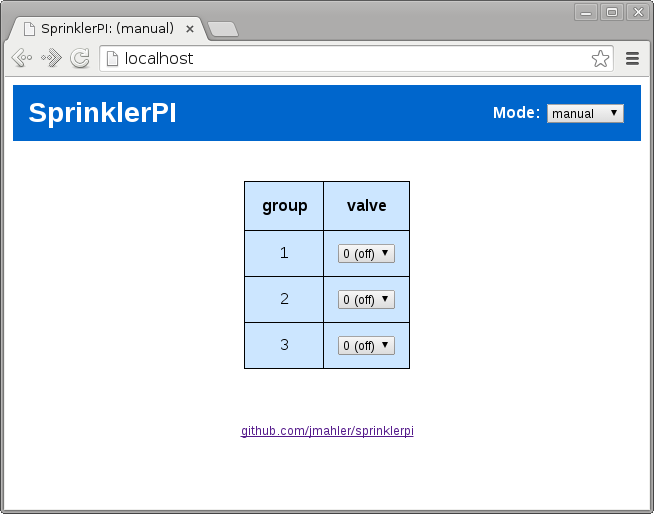
\includegraphics[scale=0.50]{../testing/img/www-manual_mode.png}
\end{center}
\caption{Web interface in manual mode.}
\label{fig:wwwmanual}
\end{figure}

\clearpage
Figure \ref{fig:wwwsched} shows the interface when in schedule mode.
From here schedules can be edit, created and enabled/disabled.
There is no practical limit on the size or complexity of these
schedules.
Notice that it is possible to start a single valve multiple times
at once.
In this case the queue daemon (Section \ref{sec:queue}) will sort
this and run the jobs for the correct amount of time although the
order is not guaranteed.

The days of the week are given in a shorthand notation
where M is Monday, T is Tuesday, W is Wednesday and so on.

The start time is specified in hours and minutes.
The run time is specified in minutes and seconds.

\begin{figure}[h!]
\begin{center}
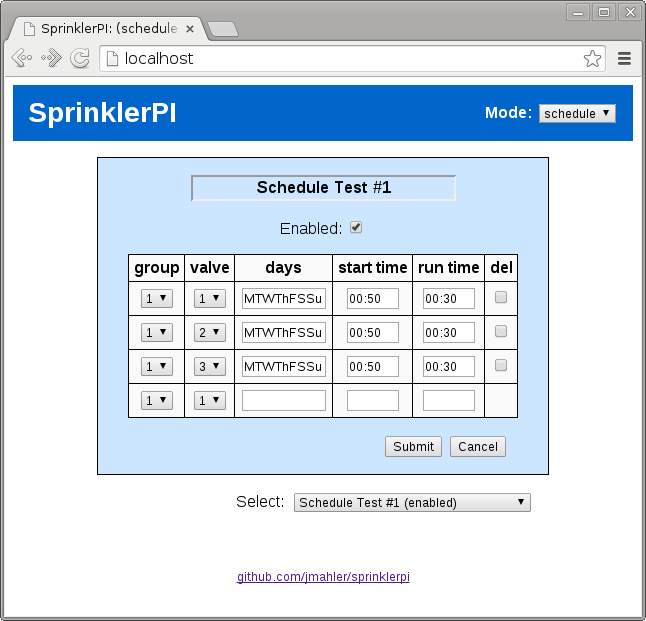
\includegraphics[scale=0.50]{../testing/img/www-schedule_test1.png}
\end{center}
\caption{Schedule interface in schedule mode.}
\label{fig:wwwsched}
\end{figure}

% }}}

\pagebreak
\glsaddall
\printglossaries

% References
\clearpage
\printbibliography[heading=bibintoc]

\end{document}
